% Chapter 2

\chapter{Literature Review} % Introduction


\label{Chapter2} % 

Analyzing event data presents its own unique challenges and questions. What are the ways to represent the data?  What types of stochastic 
models  are  appropriate  for  explaining  the  structure  in  the  data? How  can  we  measure  
how  well  the  data  is  described  by  a  particular  model?  Within literature the problem is referred to as event prediction, sequence prediction, or temporal point process modeling.

When modelled as a temporal point process, the data can be represented as a sequence of fixed period intervals in one of three ways: as an ordered list of event times ${T_i,...T_n}$, as inter-event times $U_1,...U_n$ where $u+i = T_i-T_{i-1}$, or as a counting process where  $N(t)$ is a count of the number of events occuring before time $t$ \parencite{Borgan}.

\begin{figure}[h!]
	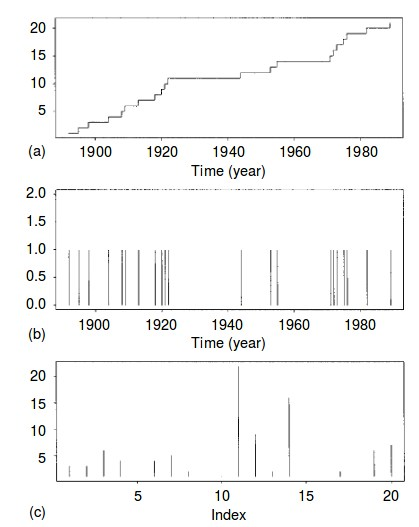
\includegraphics[width=7cm, keepaspectratio]{fig001.jpg}
	\caption{Three different representations of the same point-process a) event count b) date of occurence c) inter-event time}
	\label{fig:fig1}
\end{figure}

Of these, inter-event time is the most commonly used, for example in the times between financial transactions \parencite{EngleRusell}. An example of the counting process is the socring of goals in soccer \parencite{Heuer}. In the case of music listening, we can model a sequence of events and non-events, where $t_i$ can either be 0 (did not play music) or 1 (played music). This is the form we use in all but the Bayesian model as described in the next chapter.

\subsubsection{Conditional Intensity Function}

The conditional intensity function, $\lambda(t)$, represents the infinitesimal rate at which events are expected to occur around a particular time 
$t$, conditional on the prior history of the point 
process prior to time $t$. A Poisson process \parencite{Kingman} is a simple point process in which the probability of an event at time $t$ is assumed to be independent from all other times, and where the conditional intensity function follows a Poisson distribution based on $\lambda$. $\lambda$ may be estimated parametrically \parencite{DuWang} or via a parametric model. With the Poisson process, $\lambda$ depends only on $t$, where as in other point process models it would depends on the history preceding $t$. 
 
If the conditional intensity remains constant over time it is referred to as a homogenous or stationary point process \parencite{Nok}. If however it can vary with time it is inhomgenous, such as the self-exciting (Hawkes) process where the intensity is determined by previous events through the parametric form $\lambda(t) = \mu + \beta \sum_{t_i<t}g(t-t_i)$ and where $g$ is a non-negative kernel function. Note that the logit function used in generalized linear model, can also be thought of a conditional intensity function and has been used to develop sophisticated models such as \parencite{baddeley2014logistic} and \parencite{rajala2014note}.

However, as noted by Wass et. al \parencite{Wass}, point process models using a condictional intensity function often make various parametric assumptions about the latent dynamics governing the generation of the observed point patterns. As a consequence, model mis-specification can cause significantly degraded performance in point process models.

\subsubsection{Deep Learning}

In recent years deep learning has demonstrated the power to learn hierarchical non-linear patterns on large-scale datasets \parencite{DL} through multiple layers of abstraction (e.g. multi-layer feedforward neural networks). It has achieved state-of-the-art performances on a wide range of applications, such as computer vision \parencite{ImageNet}, natural language processing \parencite{Socher}, and protein structure prediction \parencite{Lena}.

However it has not been applied to temporal point processes until recently with Xiao et. al \parencite{Wass} applying Generative Adversarial Networks (GANS) to the problem. GANs consist of two neural network models - a generator tasked with generating (i.e. predicting) a future sequence of events based on the history, and a discriminator tasked with detecting the true (ground truth) sequence amongst the generated ones.

For measuring the loss between a generated and true sequence, the authors found the Wassertein-Distance \parencite{WassGAN} performed better than Maximum Likihood Estimate (MLE) which they remarked "may suffer from mode dropping or get stuck in an inferior local minimum".

Their findings showed that while parametric point process models work better with problems where a parametetric form exists, with real world data a GAN model with Wasserterin-Distance outperforms all other models. 

\subsection{Recurrent Neural Networks (RNN)}

RNNs are a type of artificial neural network designed to recognize patterns in sequences of data, such as text, genomes, handwriting, the spoken word, or numerical times series data emanating from sensors, stock markets and government agencies. Whilst a traditional Feed-Forward network \parencite{MLP} has input nodes, hidden layers, and an output layer, with data flowing in one direction only, RNNs allow for the hidden state from one timestep of the neural net to be an input into the next (see fig. \ref{RNN}).

\begin{figure}[h!]
	\centering
	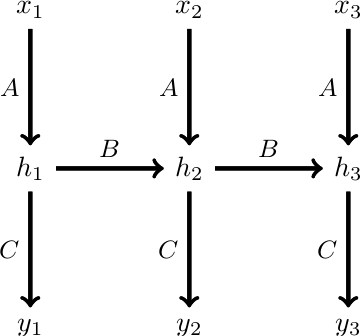
\includegraphics[width=3cm, keepaspectratio,]{fig007.jpg}
	\caption{RNN with 3 timesteps}
	\label{RNN}
\end{figure} 

RNN models can employ different methods for the propogration of the hidden state over time. One such well known method is Long Short-Term memory (LSTM) \parencite{Olah}. Here the hidden state is the product of a further four layers that interact in a way as to learn what information to retain and what information to throw away. 

\begin{figure}[h!]
	\centering
	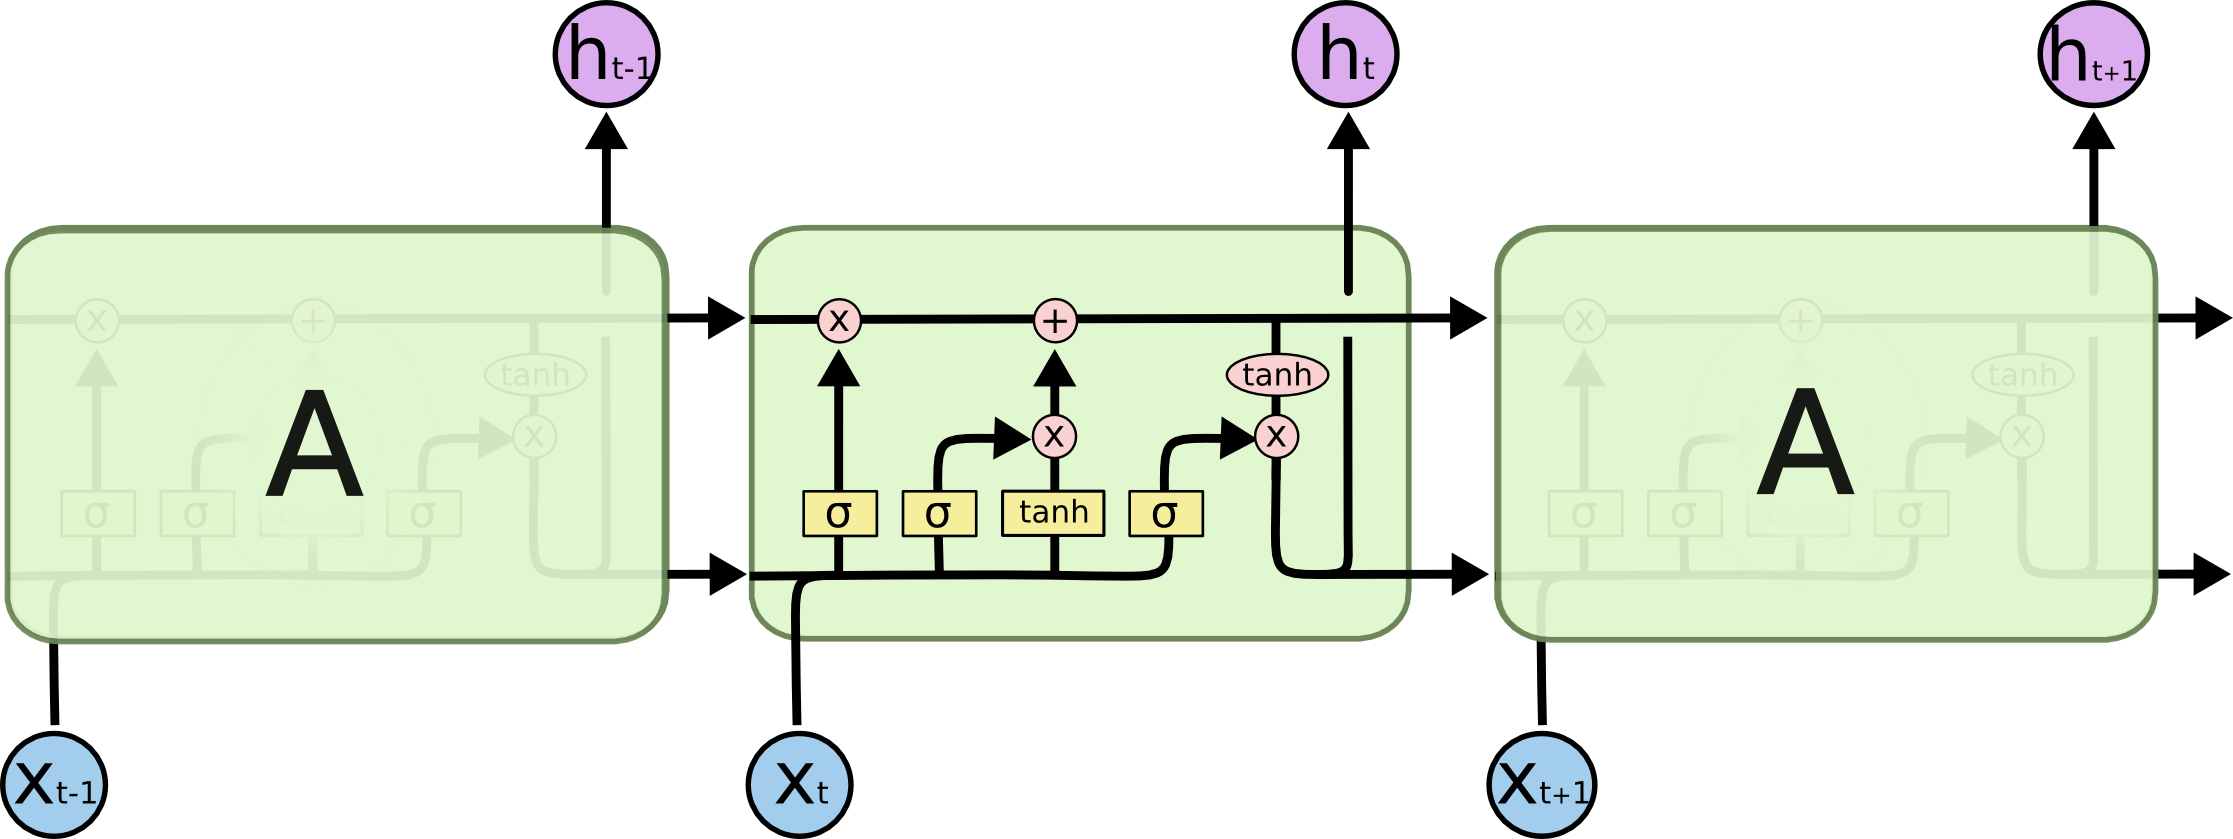
\includegraphics[width=5cm, keepaspectratio,]{fig008.png}
	\caption{LSTM}
	\label{fig:fig8}
\end{figure} 

Recently \parencite{xiao2017modeling} attempts have been made to combine concepts of temporal point processes with that of an RNN. The authors viewed the conditional intensity function of a point process as a non-linear mapping between the predicted transient occurrence intensity of events with different types, and the  model  input  information  of  event  participators, event
profile and the system history.

They model this non-linear mapping by utilizing two RNNs: one for modeling the time-series data and associated features and a second to model long-range dependency over history with arbitary time intervals; specifically a sequence of event type and the time since the previous event. In this way they can capture both the temporal based patterns, as well as the non-temporal, event-correlations which approximates to a conditional intensity function based on inter-event time.

The favoured evaluation metrics in their research were precision, recall, f1 score, and a confusion matrix, with a logistic regression model used as a baseline to compare against.

\section{Summary}

While not an exhaustive review of techniques we have seen some of the ways in which point processes can be modelled using traditional conditional intensity based models, as well as more recent areas of experimentation using deep learning. In the next chapter we layout the approach and methods we wish to explore in the context of this research.